\chapter{Conclusioni}\label{ch:conclusioni}

\section{Risultati degli esperimenti sui toy-dataset}

\subsection{Parametro k e dimensione del dataset}

\begingroup

    \begin{figure}
        \centering
        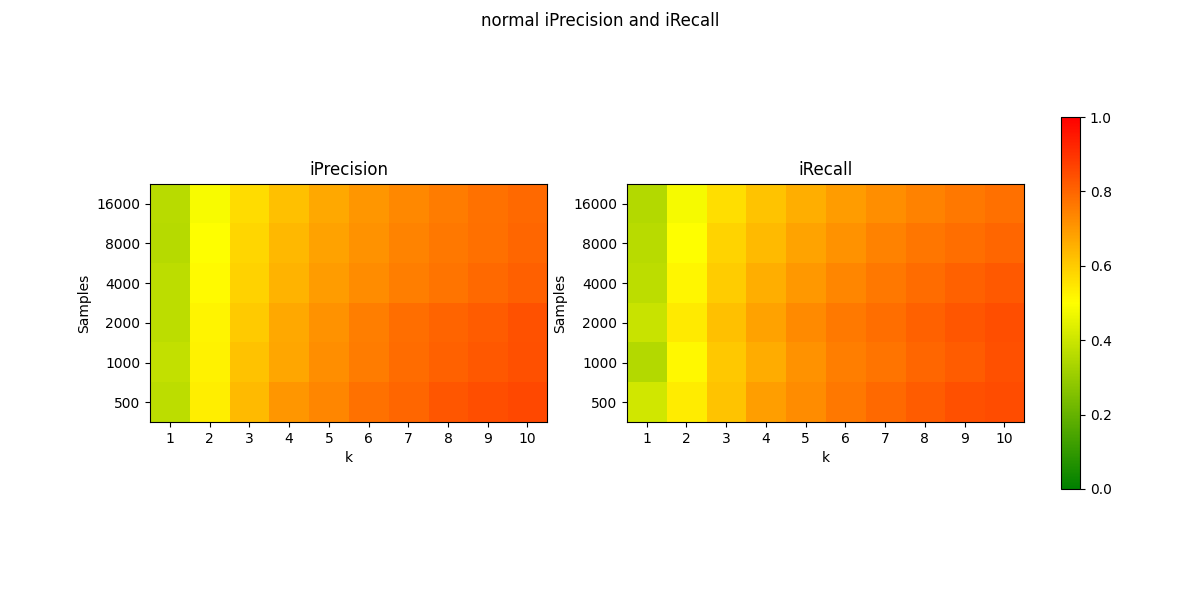
\includegraphics[width=\linewidth]{../images/toyexperiments/kdim/normal_iPrecision_iRecall.png}
    \end{figure}

    \begin{figure}
        \centering
        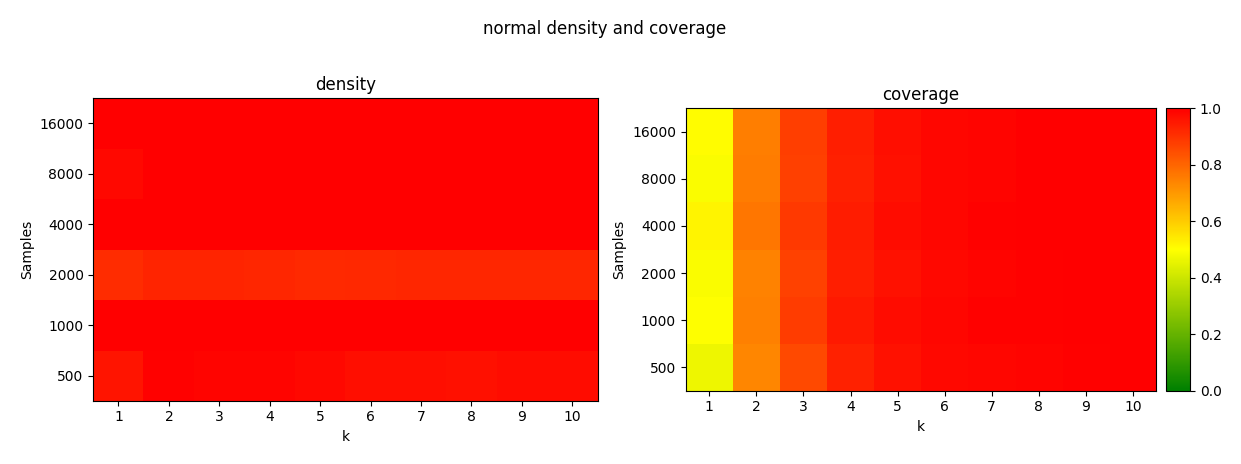
\includegraphics[width=\linewidth]{../images/toyexperiments/kdim/normal_density_coverage.png}
    \end{figure}    

    \begin{figure}
        \centering
        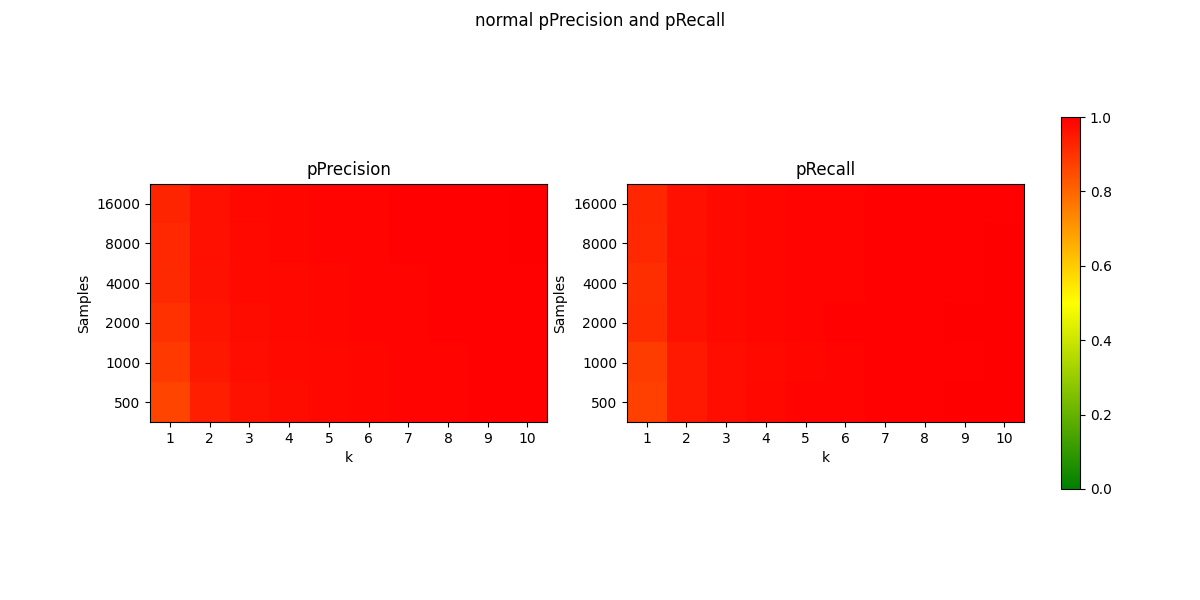
\includegraphics[width=\linewidth]{../images/toyexperiments/kdim/normal_pPrecision_pRecall.png}
    \end{figure}

    \begin{figure}
        \centering
        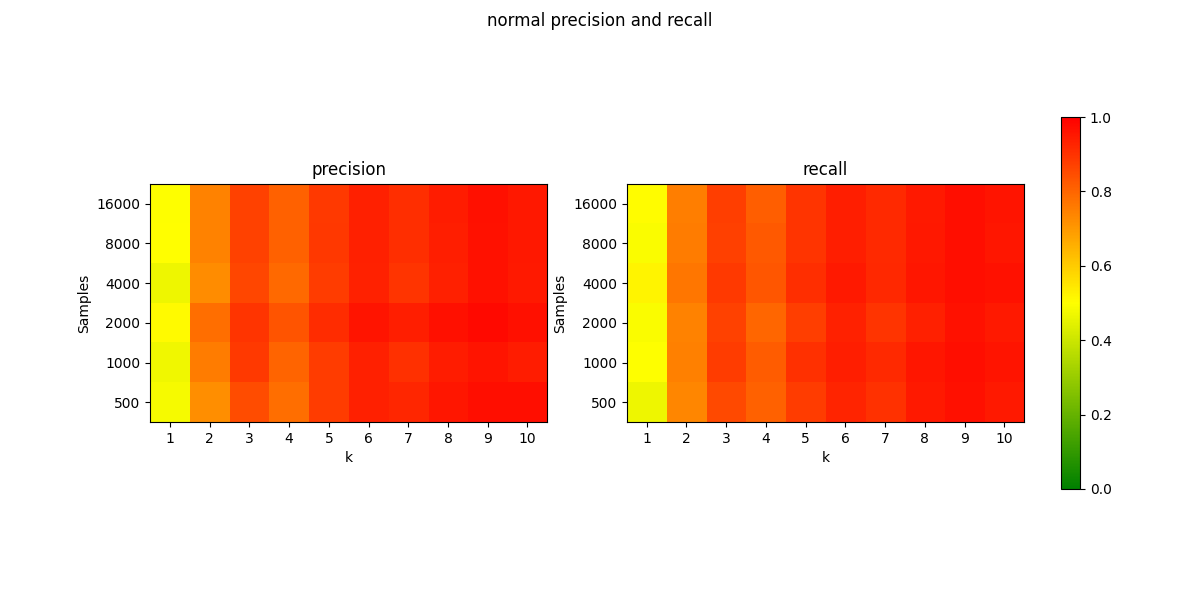
\includegraphics[width=\linewidth]{../images/toyexperiments/kdim/normal_precision_recall.png}
    \end{figure}

    \begin{figure}
        \centering
        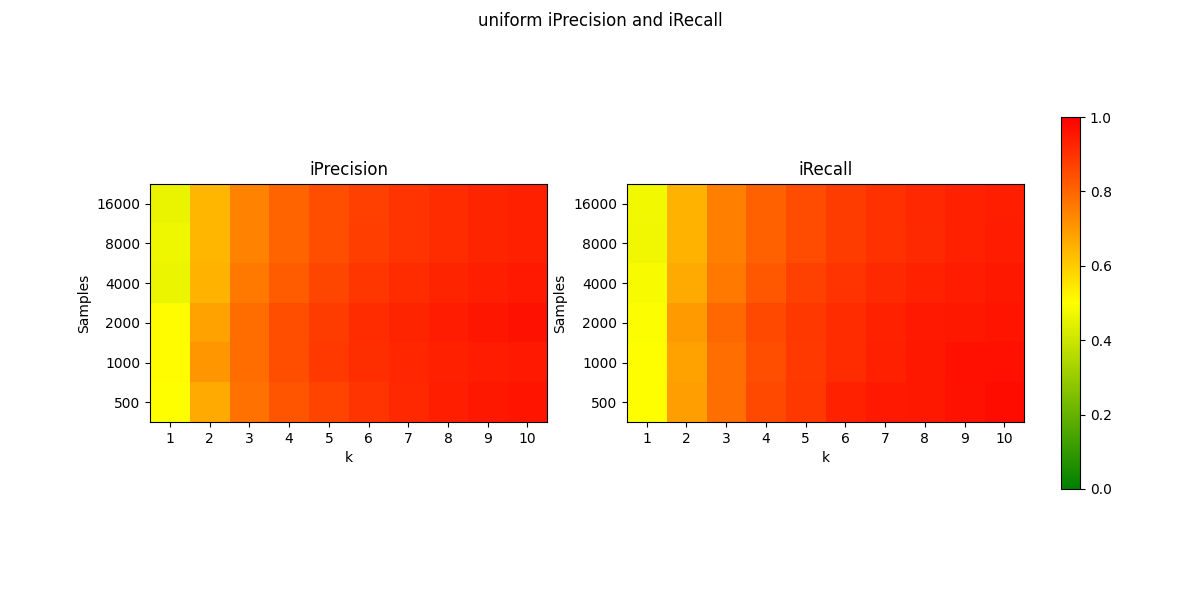
\includegraphics[width=\linewidth]{../images/toyexperiments/kdim/uniform_iPrecision_iRecall.png}
    \end{figure}

    \begin{figure}
        \centering
        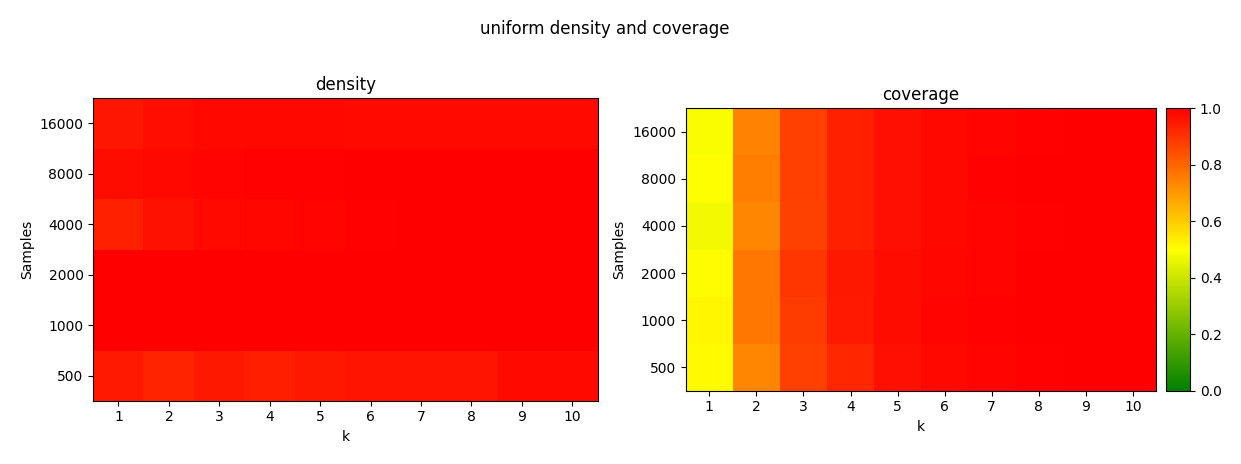
\includegraphics[width=\linewidth]{../images/toyexperiments/kdim/uniform_density_coverage.png}
    \end{figure}

    \begin{figure}
        \centering
        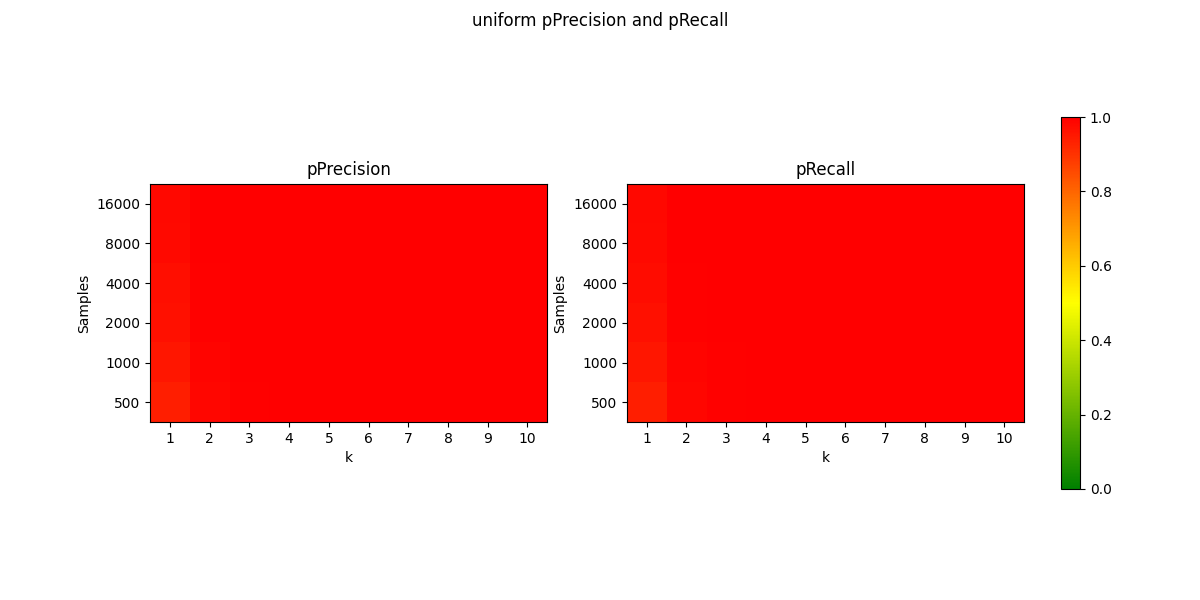
\includegraphics[width=\linewidth]{../images/toyexperiments/kdim/uniform_pPrecision_pRecall.png}
    \end{figure}

    \begin{figure}
        \centering
        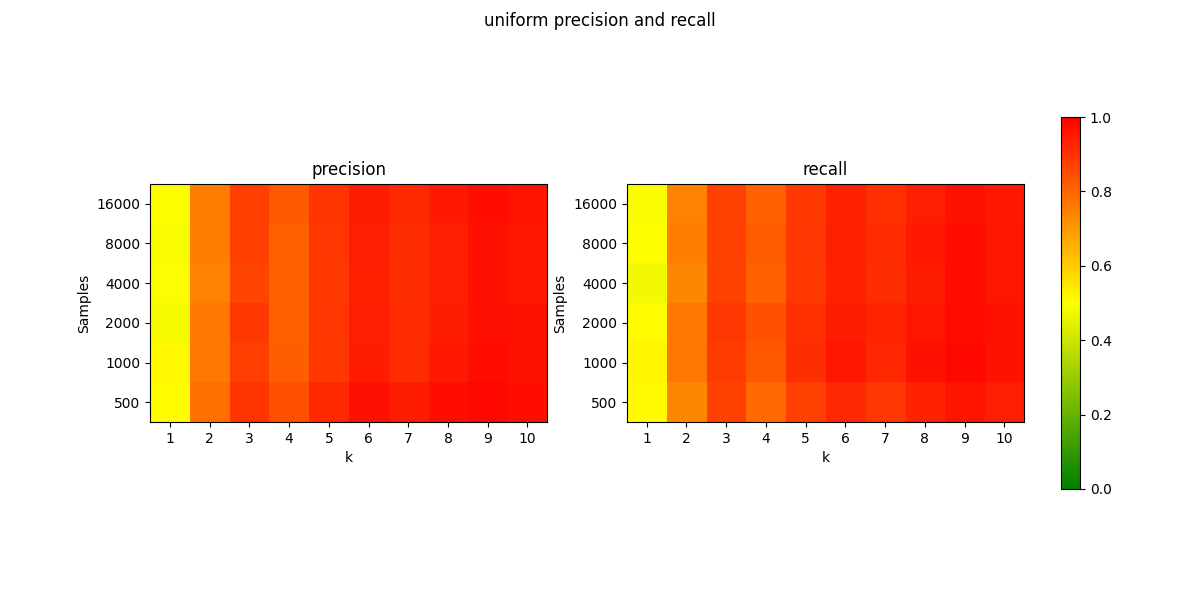
\includegraphics[width=\linewidth]{../images/toyexperiments/kdim/uniform_precision_recall.png}
    \end{figure}

\endgroup

\subsection{Dimensione del dataset e dimensione dei dati}

\begin{figure}[h!]
    \centering
    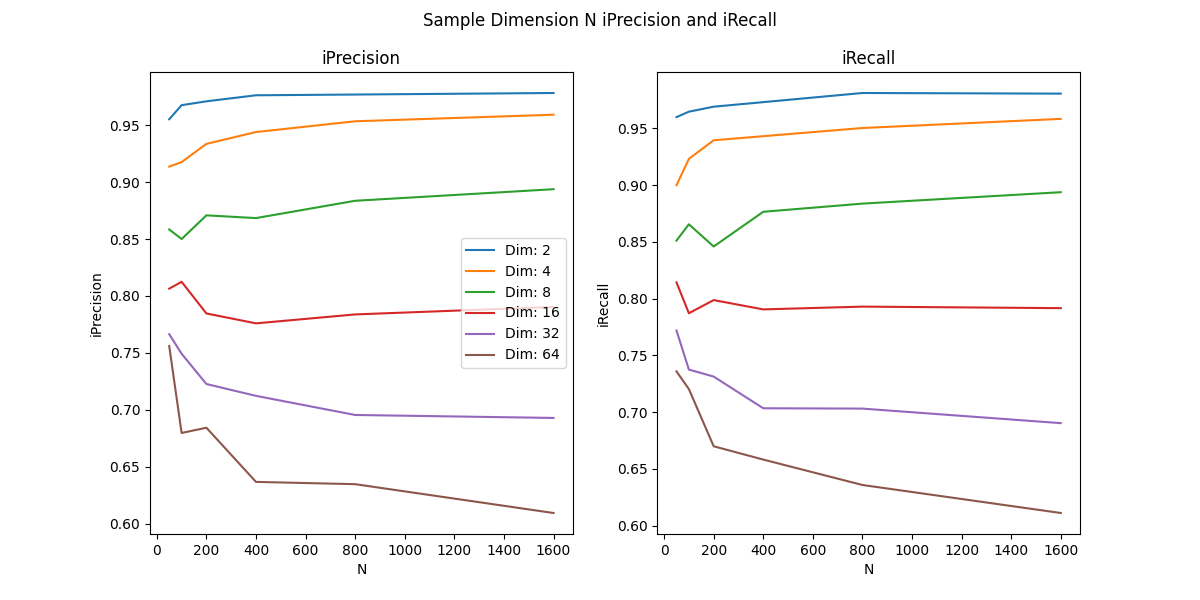
\includegraphics[width=\linewidth]{../images/toyexperiments/ksampledim/sampleDimN_iPrecision_iRecall.png} 
    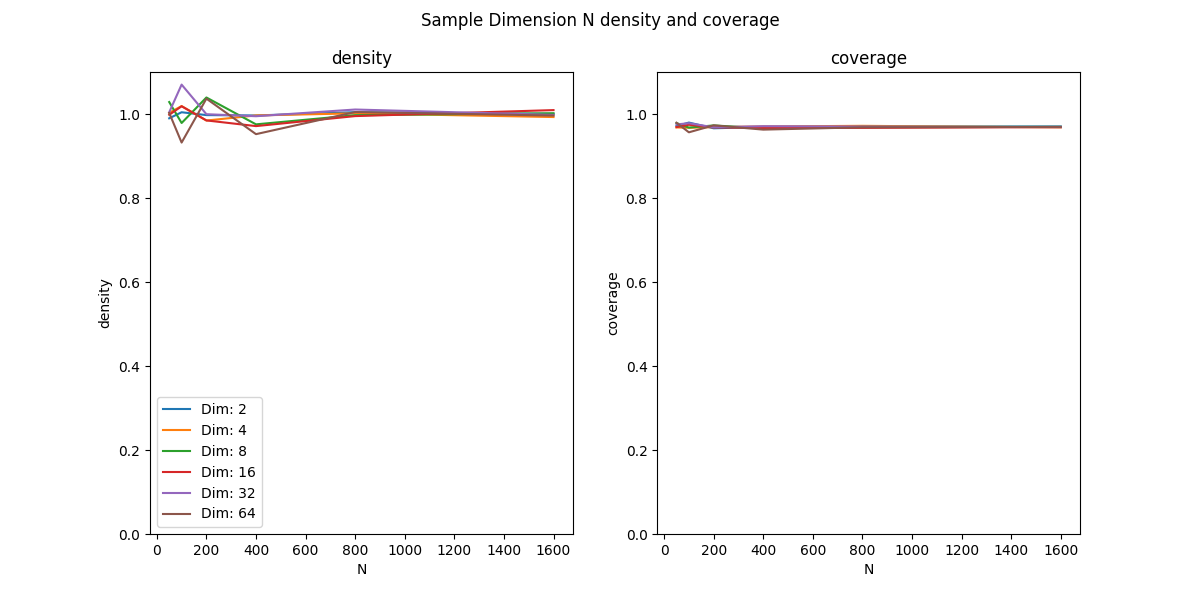
\includegraphics[width=\linewidth]{../images/toyexperiments/ksampledim/sampleDimN_density_coverage.png} 
    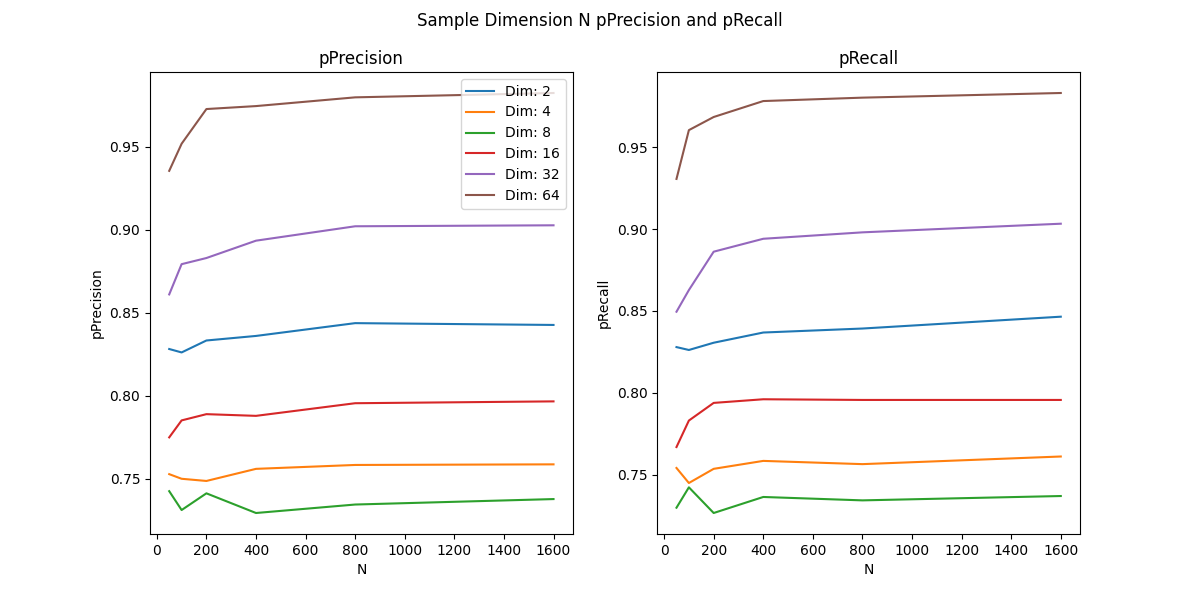
\includegraphics[width=\linewidth]{../images/toyexperiments/ksampledim/sampleDimN_pPrecision_pRecall.png} 
    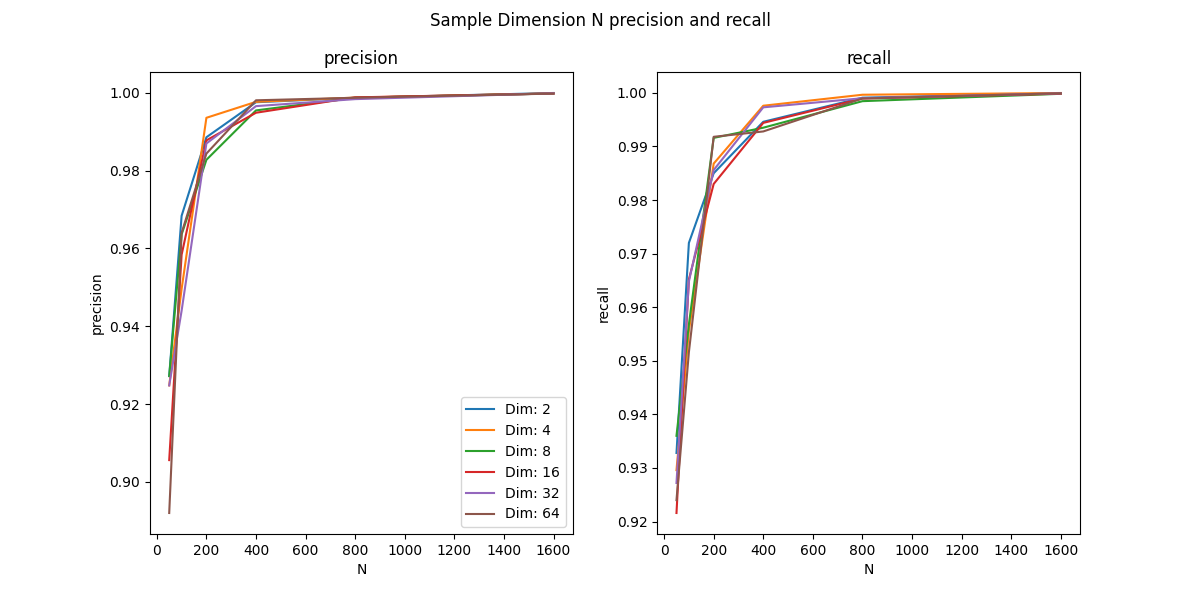
\includegraphics[width=\linewidth]{../images/toyexperiments/ksampledim/sampleDimN_precision_recall.png} 
\end{figure}

\subsection{Outliers}

\begin{figure}[h!]
    \centering
    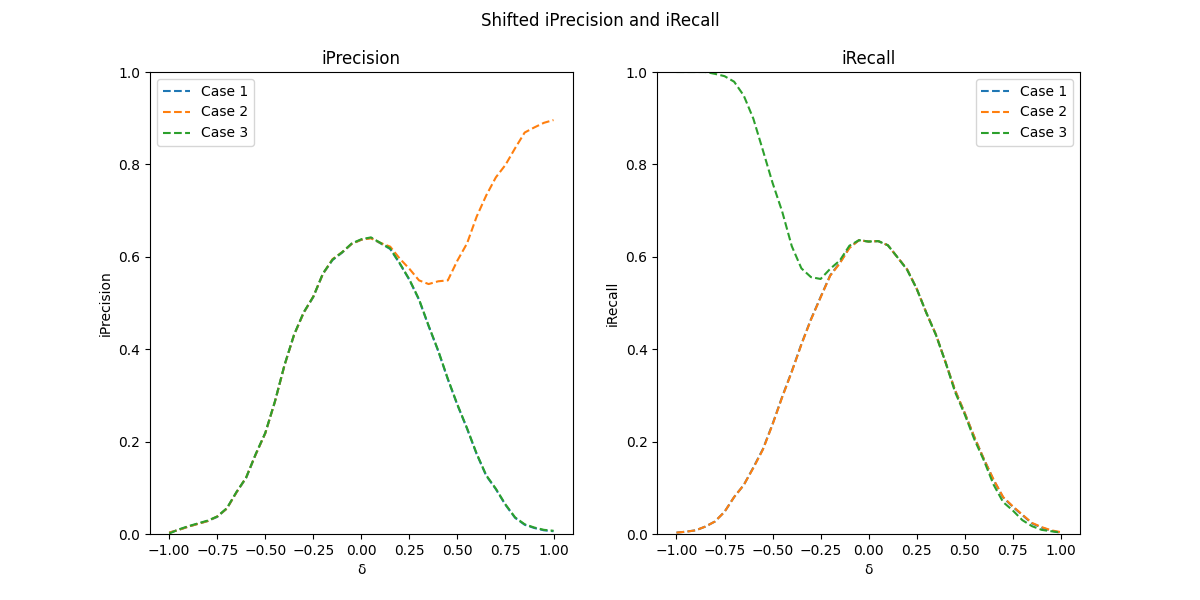
\includegraphics[width=\linewidth]{../images/toyexperiments/outliers/shift_iPrecision_iRecall.png} 
    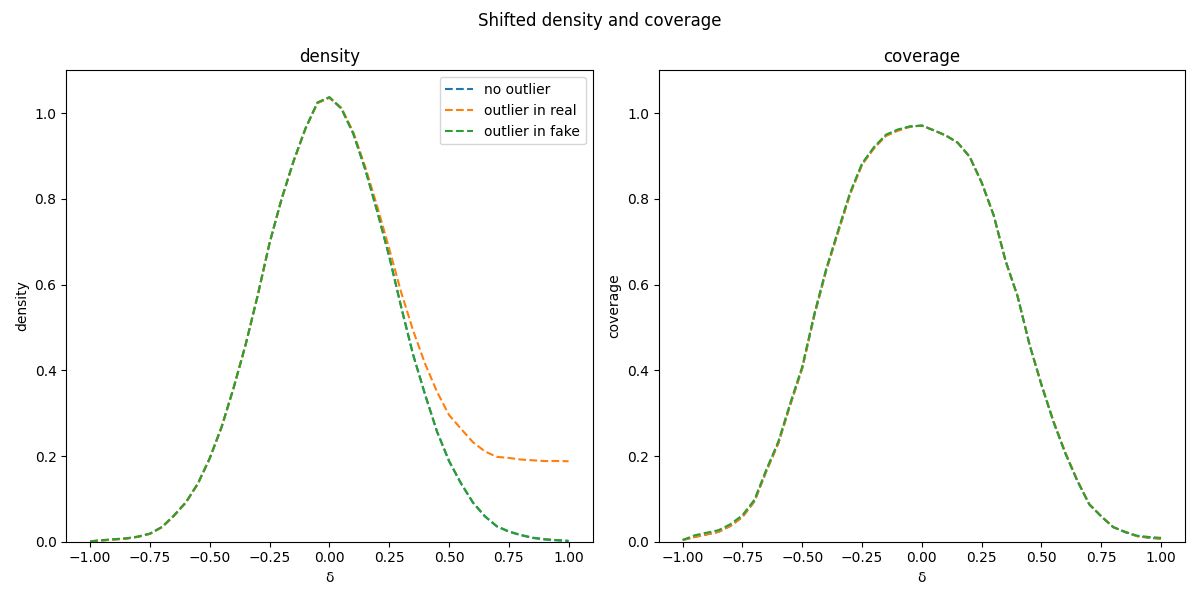
\includegraphics[width=\linewidth]{../images/toyexperiments/outliers/shift_density_coverage.png} 
    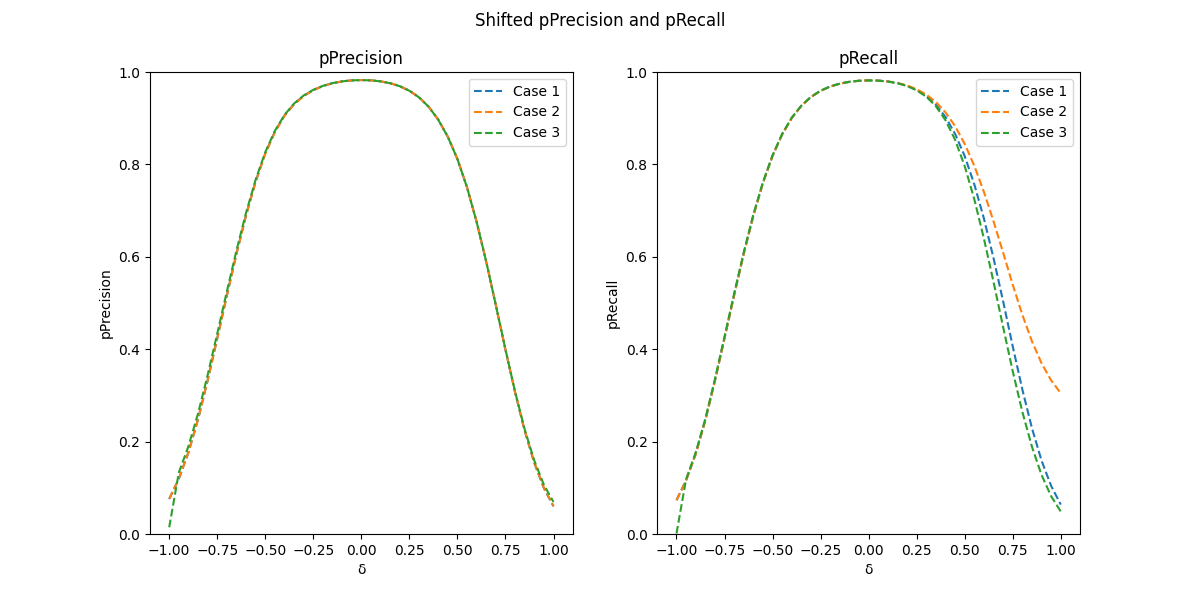
\includegraphics[width=\linewidth]{../images/toyexperiments/outliers/shift_pPrecision_pRecall.png} 
    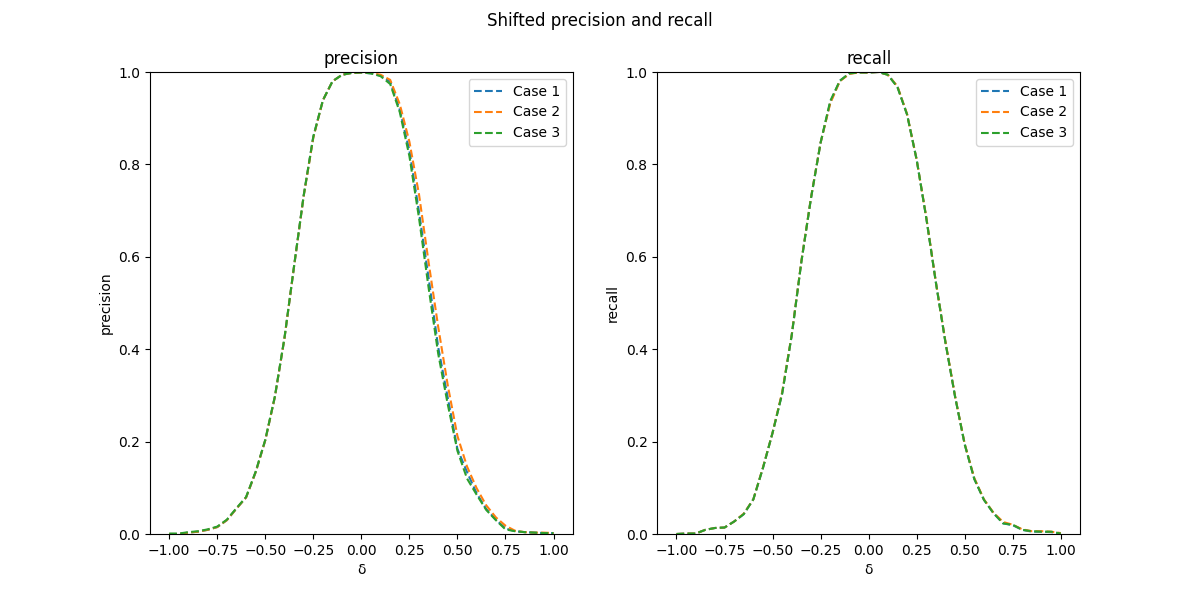
\includegraphics[width=\linewidth]{../images/toyexperiments/outliers/shift_precision_recall.png} 
\end{figure}

\subsection{Comparazione con implementazioni esistenti e riproduzione delle pr-curves}

\begin{figure}[h!]
    \centering
    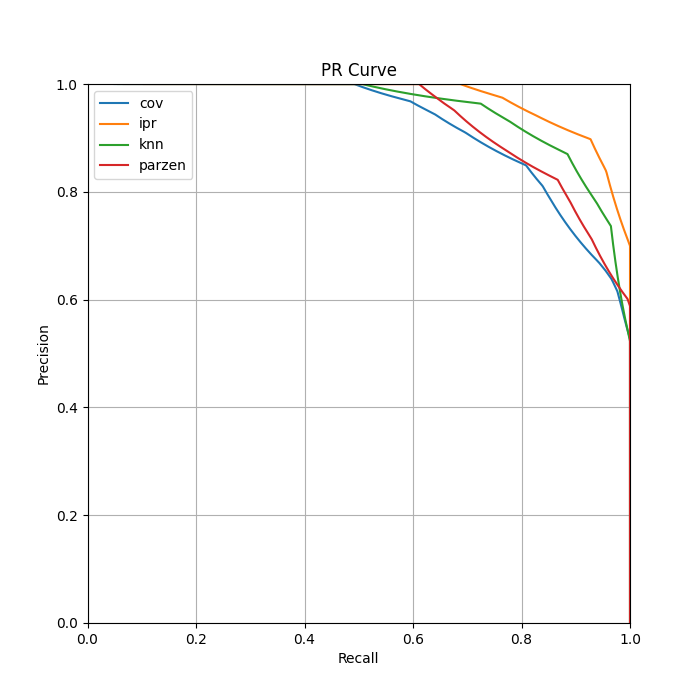
\includegraphics[width=\linewidth]{../images/toyexperiments/prcurves/PRCurve_k4_s1.png} 
    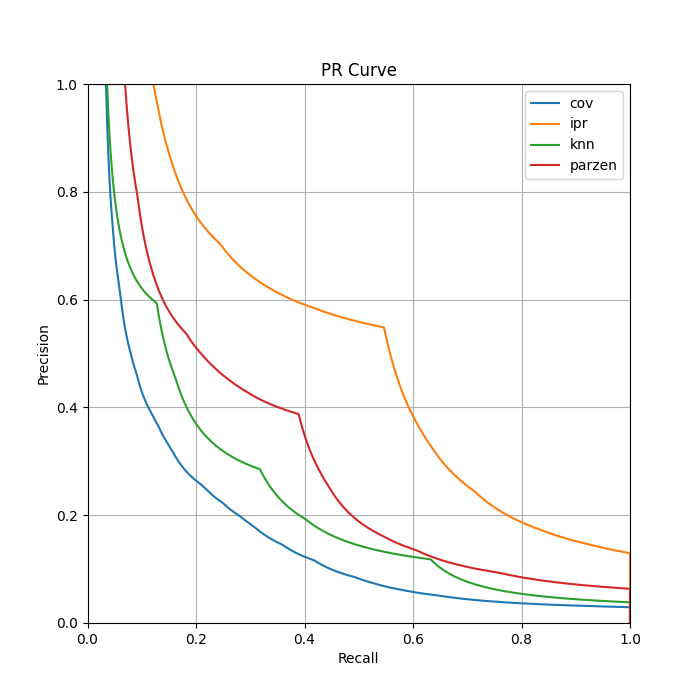
\includegraphics[width=\linewidth]{../images/toyexperiments/prcurves/PRCurve_k4_s3.png}
    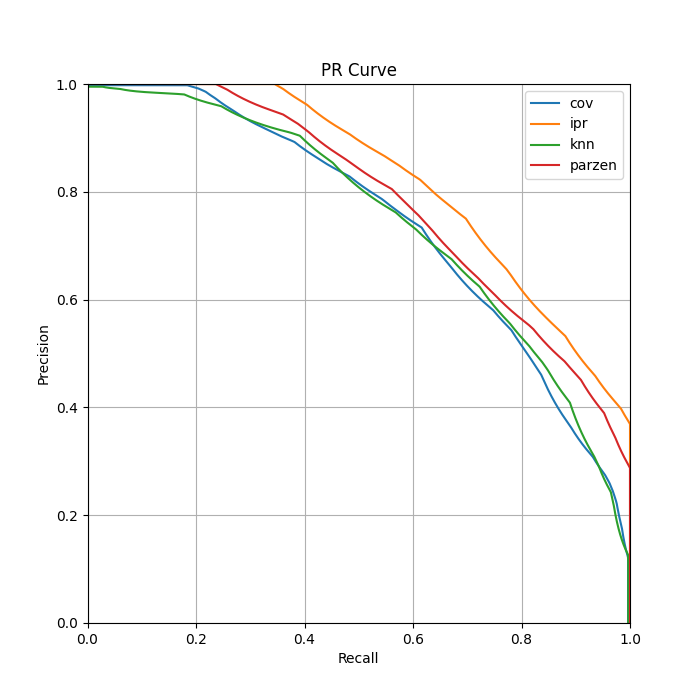
\includegraphics[width=\linewidth]{../images/toyexperiments/prcurves/PRCurve_ksqrt_s1.png} 
    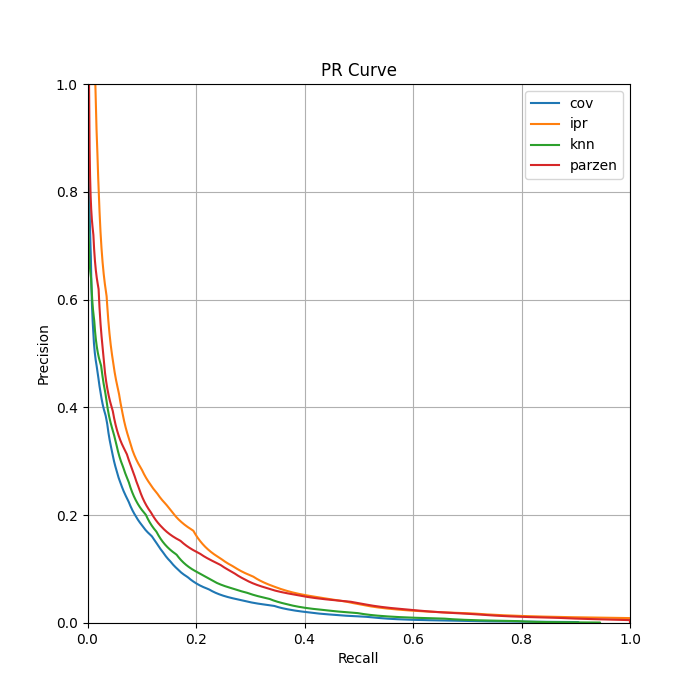
\includegraphics[width=\linewidth]{../images/toyexperiments/prcurves/PRCurve_ksqrt_s3.png} 
    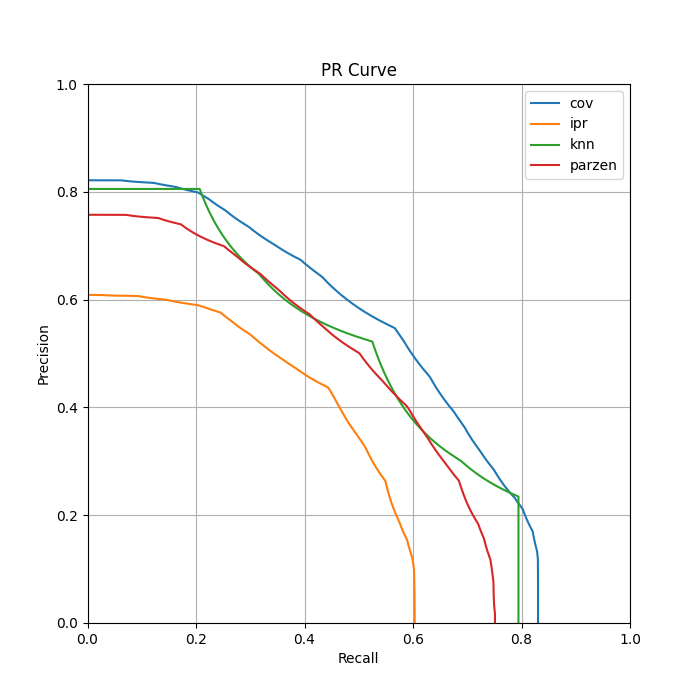
\includegraphics[width=\linewidth]{../images/toyexperiments/prcurves/PRCurve_nosplit_k4_s1.png}
    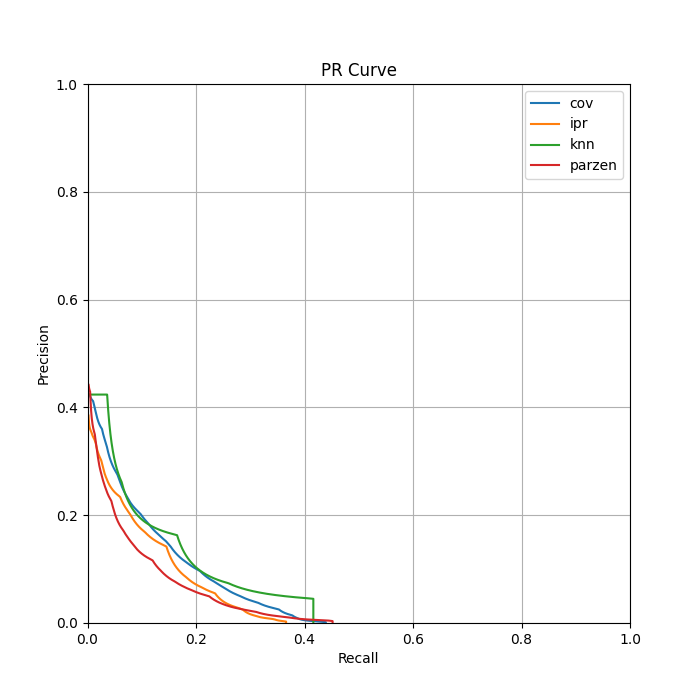
\includegraphics[width=\linewidth]{../images/toyexperiments/prcurves/PRCurve_nosplit_k4_s3.png}
    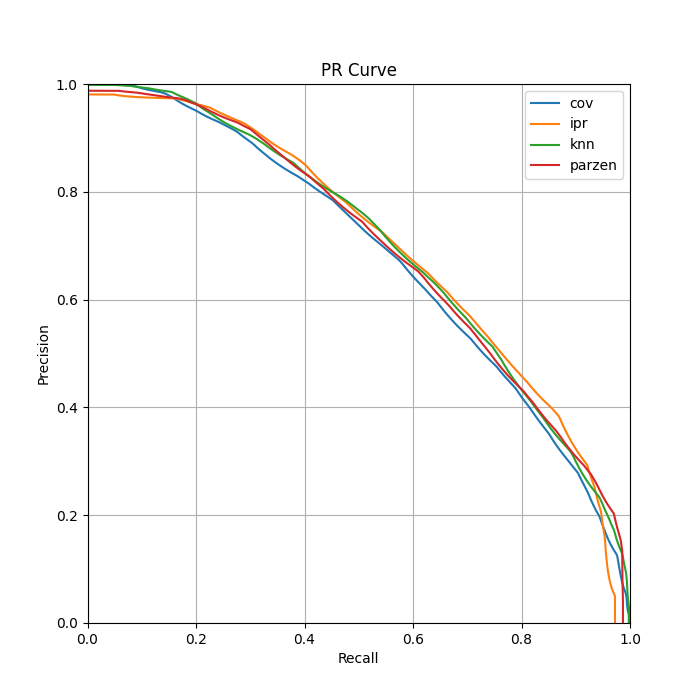
\includegraphics[width=\linewidth]{../images/toyexperiments/prcurves/PRCurve_nosplit_ksqrt_s1.png}
    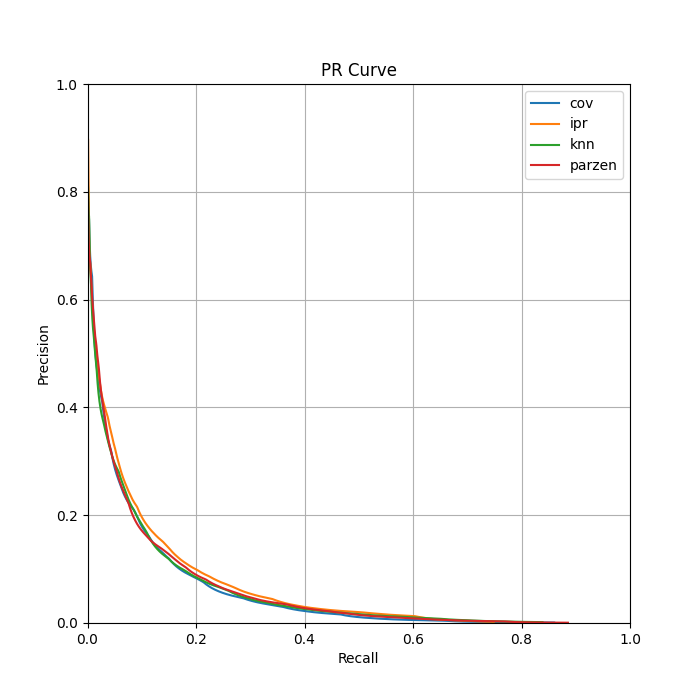
\includegraphics[width=\linewidth]{../images/toyexperiments/prcurves/PRCurve_nosplit_ksqrt_s3.png}
\end{figure}

\section{Risultati degli esperimenti su dataset reali}